\section{Algoritmo}

Utilizzando le tecniche descritte nella sezione precedente è stato ideato l'algoritmo descritto in [1].

L'algoritmo può essere suddiviso in 4 parti fondamentali:
\begin{enumerate}
\item Estrazione di features
\item Creazione di un modello a mistura di gaussiane
\item Calcolo dei \emph{tensori di fisher}
\item Classificazione
\end{enumerate}

\subsection{Estrazione delle \emph{features}}

In questa fase ciascuna scansione viene elaborata al fine di estrarre delle \emph{features}. 

Inizialmente, data un immagine viene calcolata la sua maschera, ovvero un'immagine binaria che evidenzia i pixels di \emph{foreground}. In questo modo il calcolo delle \emph{features} verrà effettuato solamente sui pixels rilevanti dell'immagine, escludendo lo sfondo.

L'immagine viene scansionata a blocchi quadrati di dimensione 80 pixels, sovrapposti con un passo di 20 pixels.

\begin{figure}[H]
\captionsetup[subfigure]{labelformat=empty}
\begin{subfigure}{.5\textwidth}
\centering
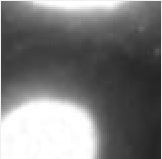
\includegraphics[height=1.6cm]{images/block.png}
\caption{Blocco}
\end{subfigure}%
\begin{subfigure}{.5\textwidth}
\centering
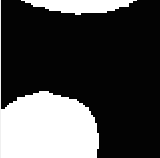
\includegraphics[height=1.8cm]{images/mask.png}
\caption{Maschera}
\end{subfigure}%
\caption{Esempio di blocco e maschera di elaborazione}
\end{figure}

